\chapter{Operational Faults}\label{operational-faults}

\section{Introduction to HVAC Operational Faults Modeling}\label{introduction-to-hvac-operational-faults}

Most of the buildings, either new or old, have operational faults in the sensors, controllers, meters, equipment and systems. Being able to model and simulate these faults and their impact on energy performance of buildings is crucial to improve accuracy of building simulations and to support the retrofit of buildings. To date, the main practitioner use of EnergyPlus has been for new construction design. With the new high priority attached by USDOE to retrofit and improved operation of existing buildings, there is a need to extend the capabilities of EnergyPlus to model existing buildings, including faulty operation:

\begin{itemize}
\tightlist
\item
  Retrofit analysis: starts with calibrated simulation; the ability to estimate the severity of common faults is expected to improve the accuracy and transparency of the calibrated model and hence the increase accuracy of the analysis of different retrofit measures.\\
\item
  Commissioning providers can use the fault models to demonstrate the saving to be expected from fixing faults found in retro-commissioning
\item
  Support for building operation by using the calibrated model, including unfixed faults, as a real-time reference model to detect, and verify the diagnosis of, newly occurring faults.
\end{itemize}

The users in these cases are practitioners, not power users, so it is needed to implement the fault models using conventional EnergyPlus objects rather than the EMS, which, in any case, could only be used to model limited types of faults.

EnergyPlus contains a number of objects to model operational faults of sensors, meters, equipment and systems. The current implementation allows the modeling of a number of fault types that categorized as: (1) sensor faults with air economizers (e.g., outdoor air temperature sensor) (2) thermostat/humidistat offset faults, (3) fouling or scaling at air side or water side components (e.g., heating and cooling coil, air filter, cooling tower), (4) sensor faults with plant components (e.g., chiller supply water temperature sensor offset).


\section{Operational Faults Modeling}\label{operational-faults-modeling}

\subsection{Sensor Faults with Air Economizers}\label{sensor-faults-with-air-economizers}

\subsubsection{Symptom}\label{symptom}

The sensor readings deviate from the actual air conditions due to sensor offset, which leads to inappropriate operations of the air economizer and thus undesired resulting indoor conditions.

\subsubsection{Modeling Approach}\label{modeling-approach}

There are a number of sensors installed to support the air economizer operations. The sensors may be of different types. The objects used by EnergyPlus to model the sensor faults are as follows:

\begin{itemize}
\tightlist
\item
  FaultModel:TemperatureSensorOffset:OutdoorAir
\item
  FaultModel:HumiditySensorOffset:OutdoorAir
\item
  FaultModel:EnthalpySensorOffset:OutdoorAir
\item
  FaultModel:TemperatureSensorOffset:ReturnAir
\item
  FaultModel:EnthalpySensorOffset:ReturnAir
\end{itemize}

\subsection{Thermostat/Humidistat Offset}\label{thermostathumidistat-offset}

\subsubsection{Symptom}\label{symptom-1}

The zone air temperature/relative humidity readings deviate from the actual zone air conditions due to thermostat/humidistat offset, and thus leads to inappropriate operations of the HVAC system and undesired resulting indoor conditions.

\subsubsection{Modeling Approach}\label{modeling-approach-1}

The thermostat offset fault is described in the object FaultModel:ThermostatOffset, which refers to the object ZoneControl:Thermostat. The humidistat offset fault is described in the object FaultModel:HumidistatOffset, which refers to the object ZoneControl:Humidistat. The effect of an offset in a thermostat/humidistat whose sole use is for the calculation of difference between the set-points and the design values can be modeled as an equal and opposite offset in the thermostat/humidistat:

\begin{equation}
T_{s,f} = T_{s,ff}  - \Delta T
\end{equation}

\begin{equation}
RH_{s,f} = RH_{s,ff}  - \Delta RH
\end{equation}

Where,

\(T_{s,f}\) thermostat value in the faulty case, C

\(T_{s,ff}\) thermostat value in the fault-free case (design value), C

\(RH_{s,f}\) humidistat value in the faulty case,

\(RH_{s,ff}\) humidistat value in the fault-free case (design value),

\(\Delta T / \Delta RH\) difference between the thermostat/humidistat readings and the actual zone air conditions. Positive values mean that the readings is higher than the actual air conditions.

For the humidistat that is independent of the thermostat, \(\Delta RH\) can be described by a pre-defined schedule. For the humidistat offset that is caused by the thermostat offset, \(\Delta RH\) is related with both the thermostat offset level as well as the indoor air conditions which are dynamic, and therefore cannot be described with a pre-defined schedule. In this case, the humidistat offset level is calculated each time step.

\begin{equation}
\Delta RH = RH_{s,ff} - f(T_{real}, W_{s,f})
\end{equation}

Where,

\(T_{real}\) real-time temperature of the indoor air (real value), C

\(W_{s,f}\) humidistat ratio corresponding to \(T_{real} - \Delta T and RH_{s,ff, kgWater/kgDryAir}\)

Note that the thermostat/humidistat settings are related with two major processes within EnergyPlus: one is the design load calculations and HVAC system sizing, and the other is the HVAC system operations. Only the latter is affected by the thermostat/humidistat offset fault, while the former is not. Therefore, the size of the corresponding HVAC equipment in the faulty cases is the same as that in the fault-free cases.

When EMS is used to overwrite the ZoneControl:Thermostat/ZoneControl:Humidistat values, the offsets are applied to the EMS values rather than the original Thermostat/Humidistat values.

\subsection{Heating and Cooling Coil Fouling}\label{heating-and-cooling-coil-fouling}

\subsubsection{Symptom}\label{symptom-2}

Reduced overall heat transfer coefficient (UA) causes reduced coil capacity, resulting in unmet loads and/or increased water flow rate and decreased water side temperature difference (``low ΔT'' syndrome).

\subsubsection{Modeling Approach}\label{modeling-approach-2}

The coil fouling fault is described in the object FaultModel:Fouling:Coil. The fault model currently applies only to the `simple' water coils: Coil:Heating:Water and Coil:Cooling:Water. The FaultModel:Fouling:Coil object allows the user to describe the fouling information in either of the two methods: FouledUARated or FoulingFactor. Using FouledUARated method, user specifies the value of UAfouled directly. Using FoulingFactor method user specifies air/water side fouling factor, and the UAfouled value is further calculated via the equations shown below.

\begin{equation}
UA_{fouled} = [UA_{air} - 1  +  R_{foul}  + UA_{water} - 1]-1
\end{equation}

Where,

\(U_{Aair}\) heat transfer coefficient of the coil on the air side, W/K

\(UA_{fouled}\) overall heat transfer coefficient of the fouled coil, W/K

\(UA_{water}\) heat transfer coefficient of the coil on the water side, W/K

\(R_{foul}\) fouling factor, K/W

\(R_{foul}\) is determined by:

\begin{equation}
R_{foul} = r_{air}/A_{air} + r_{water} / A_{water}
\end{equation}

Where,

\(r_{air}\) Air side fouling factor, m2-K/W

\(r_{water}\) Water side fouling factor, m2-K/W

\(A_{air}\) Air side coil surface area, m2

\(A_{water}\) Water side coil surface area, m2

The pressure drop associated with the fouling is ignored in the current implementation.

\subsection{Air Filter Fouling}\label{air-filter-fouling}

\subsubsection{Symptom}\label{symptom-3}

Increased air loop system resistance, resulting in a different system curve. This directly affects the operation of corresponding fans. More specifically, it may lead to variations of the fan pressure rise, fan energy consumption, as well as the enthalpy of the fan outlet air. It may also lead to a reduction in the airflow rate and thus affects the performance of other system components (e.g., heat transfer performance of heating/cooling coils).

\subsubsection{Modeling Approach}\label{modeling-approach-3}

The fouling air filter fault is described in the object FaultModel:Fouling:AirFilter, which refers to the fan objects that describe the associated fan. The fan object can be Fan:ConstantVolume, Fan:OnOff, or Fan:VariableVolume. The design pressure rise variations of the associated fan in the faulty cases are described by the Pressure Fraction Schedule specified in FaultModel:Fouling:AirFilter object, which is used as a multiplier to the fault-free fan design pressure rise specified in the fan object. The variations of the design air flow rate of the fan can then be calculated with the Pressure Fraction Schedule and Fan Curve. When EMS is used to overwrite the the pressure/MassFlow, the EMS values are used.

The effect of the fouling air filter on the fan performance is related with a number of factors, including the fan types, fan curves, and system design and operating conditions. In general, there are three possible situations to be addressed in modeling dirty air filters:

\textbf{(a) The required airflow rate can be maintained by the variable speed fan running at higher speed.}

In this case, the fan operation state changes from point A (intersection of the fan curve corresponding to a lower speed and the system curve with clean filters) to point B (intersection of the fan curve corresponding to a higher speed and the system curve with dirty filters), as shown in Figure~\ref{fig:effect-of-dirty-air-filter-on-variable-speed}. Point B corresponds to a higher fan pressure rise than Point A, and the same air flow rate.

\begin{figure}[hbtp] % fig 345
\centering
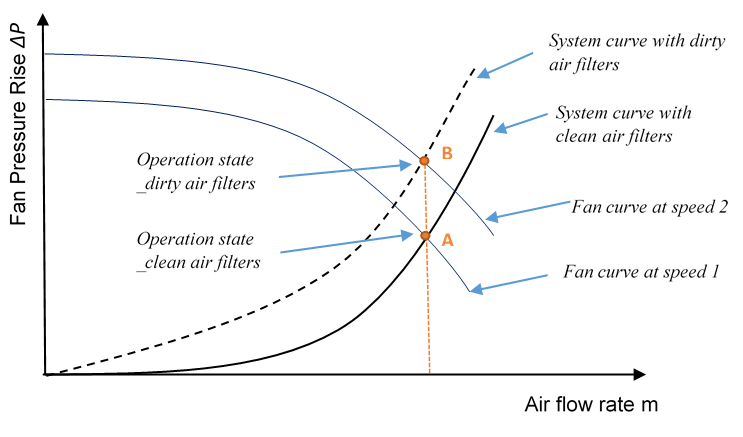
\includegraphics[width=0.9\textwidth, height=0.9\textheight, keepaspectratio=true]{media/image8006.png}
\caption{Effect of dirty air filter on variable speed fan operation – flow rate maintained \protect \label{fig:effect-of-dirty-air-filter-on-variable-speed}}
\end{figure}

The required airflow rate m can be maintained while the fan pressure rise \(\Delta P\) is increased to \(\Delta P_{df}\) . This leads to higher fan power \(\dot Q_{tot,df}\) and higher power entering the air \(\dot Q_{toair,df}\) , and thus changes the specific enthalpies of the fan outlet air stream (\(h_{out,df}\) ).

\begin{equation}
f_{flow,df} = m / m_{design,df}
\end{equation}

\begin{equation}
f_{pl,df} = c_{1} + c_{2}*f_{flow,df} + c_{3}*f_{flow,df}^2 + c_{4}*f_{flow,df}^3 + c_{5}*f_{flow,df}^4
\end{equation}

\begin{equation}
\dot{Q}_{tot,df} = f_{pl,df} \times m_{design,df} \times \Delta P_{df} / (e_{tot} \times \rho_{air} )
\end{equation}

\begin{equation}
\dot{Q}_{shaft,df} = e_{motor} \times \dot{Q}_{tot, df}
\end{equation}

\begin{equation}
\dot{Q}_{toair,df} = \dot{Q}_{shaft,df} +( \dot{Q}_{tot,df} - \dot{Q}_{shaft,df}) \times f_{motortoair}
\end{equation}

\begin{equation}
h_{out,df} = h_{in} + \dot{Q}_{toair,df} / m
\end{equation}

Where,

\(e_{tot}\) is the motor efficiency;

\(f_{flow}\) is the flow fraction or part-load ratio;

\(f_{pl}\) is the part load factor;

\(m\) is the air mass flow in kg/s;

\(h_{in}\) is the inlet air stream specific enthalpies in J/kg;

\(h_{out}\) is the outlet air stream specific enthalpies in J/kg;

\(\dot{Q}_{tot}\) is the fan power in watts;

\(\dot{Q}_{toair}\) is the power entering the air in watts;

\(\dot{Q}_{shaft}\) is the fan shaft power in watts;

\(\Delta P\) is the fan pressure increase in Pascal;

\(_{design}\) is for the parameters in the design condition;

\(_{df}\) is for the parameters in the dirty filter case.

\textbf{(b) The variable speed fan cannot increase in speed sufficiently to maintain the required airflow rate.}

In this case, the fan operation state changes from point A (intersection of the fan curve corresponding to a lower speed and the system curve with clean filters) to point B (intersection of the fan curve corresponding to a higher speed and the system curve with dirty filters), as shown in Figure~\ref{fig:effect-of-dirty-air-filter-on-variable-speed-001}. Point B corresponds to a higher fan pressure rise and a lower air flow rate than Point A.

\begin{figure}[hbtp] % fig 346
\centering
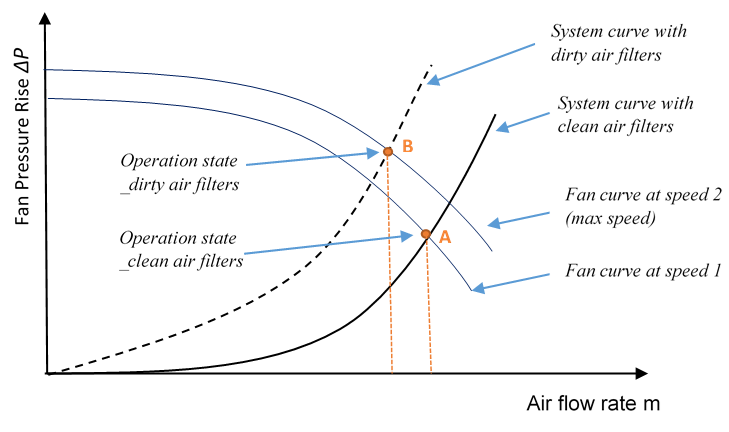
\includegraphics[width=0.9\textwidth, height=0.9\textheight, keepaspectratio=true]{media/image8007.png}
\caption{Effect of dirty air filter on variable speed fan operation – flow rate reduced \protect \label{fig:effect-of-dirty-air-filter-on-variable-speed-001}}
\end{figure}

The airflow rate m is reduced to \(m_{df}\) while the fan design pressure rise \(\Delta P\) is increased to \(\Delta P_{df}\). Similarly to case (a), the fan power (\(\dot Q_{tot}\) ), the power entering the air (\(\dot Q_{toair}\) ), and the specific enthalpies of the fan outlet air stream (\(h_{out}\) ) are all affected. Different from case (a), however, the fan power (\(\dot Q_{tot}\) ) may either increase or decrease, depending on the degree of the airflow rate decrease and pressure rise increase. Also note that \(f_{flow,df}\) is always 1 in this case, since the fan runs at its maximum speed.

\begin{equation}
f_{flow,df} = 1
\end{equation}

\begin{equation}
f_{pl,df} = c_{1} + c_{2}*f_{flow,df} + c_{3}*f_{flow,df}^2 + c_{4}*f_{flow,df}^3 + c_{5}*f_{flow,df}^4
\end{equation}

\begin{equation}
\dot{Q}_{tot,df} = f_{pl,df} \times m_{design,df} \times \Delta P_{df} / (e_{tot} \times \rho_{air} )
\end{equation}

\begin{equation}
\dot{Q}_{shaft,df} = e_{motor} \times \dot{Q}_{tot, df}
\end{equation}

\begin{equation}
\dot{Q}_{toair,df} = \dot{Q}_{shaft,df} +( \dot{Q}_{tot,df} - \dot{Q}_{shaft,df}) \times f_{motortoair}
\end{equation}

\begin{equation}
h_{out,df} = h_{in} + \dot{Q}_{toair,df} / m_{design,df}
\end{equation}

Where,

\(e_{tot}\) is the motor efficiency;

\(f_{flow}\) is the flow fraction or part-load ratio;

\(f_{pl}\) is the part load factor;

\(m\) is the air mass flow in kg/s;

\(h_{in}\) is the inlet air stream specific enthalpies in J/kg;

\(h_{out}\) is the outlet air stream specific enthalpies in J/kg;

\(\dot{Q}_{tot}\) is the fan power in watts;

\(\dot{Q}_{toair}\) is the power entering the air in watts;

\(\dot{Q}_{shaft}\) is the fan shaft power in watts;

\(\Delta P\) is the fan pressure increase in Pascal;

\(_{design}\) is for the parameters in the design condition;

\(_{df}\) is for the parameters in the dirty filter case.

\textbf{(c) The constant speed fan cannot maintain the design airflow rate.}

In this case, the fan operation state changes from point A (intersection of the fan curve and the system curve with clean filters) to point B (intersection of the fan curve and the system curve with dirty filters), as shown in Figure~\ref{fig:effect-of-dirty-air-filter-on-constant-speed}. Point B corresponds to a higher fan pressure rise and a lower air flow rate than Point A.

\begin{figure}[hbtp] % fig 347
\centering
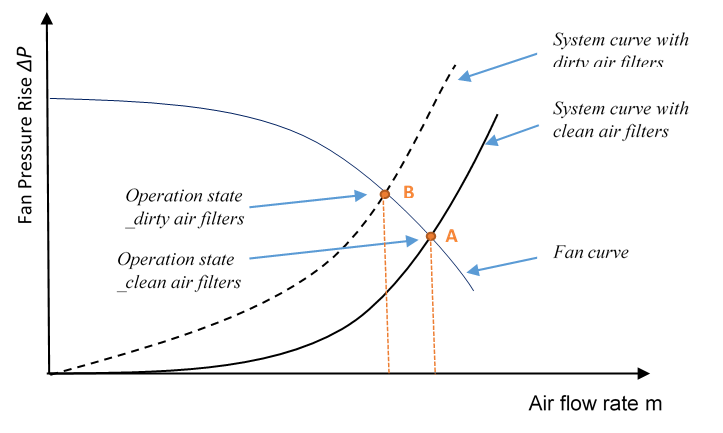
\includegraphics[width=0.9\textwidth, height=0.9\textheight, keepaspectratio=true]{media/image8008.png}
\caption{Effect of dirty air filter on constant speed fan operation \protect \label{fig:effect-of-dirty-air-filter-on-constant-speed}}
\end{figure}

Similarly to case (b), the airflow rate m is reduced to \(m_{df}\) while the fan pressure rise \(\Delta P\) is increased to \(\Delta P_{df}\) . This results in the variations of the fan power (\(\dot Q_{tot}\) ), the power entering the air (\(\dot Q_{toair}\) ), and the specific enthalpies of the fan outlet air stream (\(h_{out}\) ).

\begin{equation}
\dot{Q}_{tot,df} = m_{design,df} \times \Delta P_{df} / (e_{tot} \times \rho_{air} )
\end{equation}

\begin{equation}
\dot{Q}_{shaft,df} = e_{motor} \times \dot{Q}_{tot, df}
\end{equation}

\begin{equation}
\dot{Q}_{toair,df} = \dot{Q}_{shaft,df} +( \dot{Q}_{tot,df} - \dot{Q}_{shaft,df}) \times f_{motortoair}
\end{equation}

\begin{equation}
h_{out,df} = h_{in} + \dot{Q}_{toair,df} / m_{design,df}
\end{equation}

Where,

\(e_{tot}\) is the motor efficiency;

\(m\) is the air mass flow in kg/s;

\(h_{in}\) is the inlet air stream specific enthalpies in J/kg;

\(h_{out}\) is the outlet air stream specific enthalpies in J/kg;

\(\dot{Q}_{tot}\) is the fan power in watts;

\(\dot{Q}_{toair}\) is the power entering the air in watts;

\(\dot{Q}_{shaft}\) is the fan shaft power in watts;

\(\Delta P\) is the fan pressure increase in Pascal;

\(_{design}\) is for the parameters in the design condition;

\(_{df}\) is for the parameters in the dirty filter case.


\subsection{Chiller Supply Water Temperature Sensor Offset}\label{chiller-supply-water-temperature-sensor-offset}

\subsubsection{Symptom}

The chiller supply water temperature readings deviate from the actual water temperature levels due to sensor offset at the evaporator outlet. This can lead to incorrect chiller supply water temperature, and thus the inappropriate and inefficient chiller operations.

\subsubsection{Modeling Approach}

The fault applies to a number of chiller types, namely:

\begin{itemize}
\tightlist
\item
  Chiller:Electric
\item
  Chiller:Electric:EIR
\item
  Chiller:Electric:ReformulatedEIR
\item
  Chiller:ConstantCOP
\item
  Chiller:EngineDriven
\item
  Chiller:CombustionTurbine
\item
  Chiller:Absorption
\item
  Chiller:Absorption:Indirect
\end{itemize}

These chillers can have different flow modes:

\begin{itemize}
\tightlist
\item
  \emph{ConstantFlow} for constant pumping with flow controlled by chiller to operate at full design flow rate.
\item
  \emph{LeavingSetpointModulated} for variable pumping with flow controlled by chiller to vary flow to target a leaving temperature setpoint.
\item
  \emph{NotModulated} for either variable or constant pumping with flow controlled by the external plant system.
\end{itemize}

\textbf{(a) constant flow chillers}

For the chillers with \emph{ConstantFlow} and \emph{NotModulated}, local control is provided by resetting the leaving water temperature. The actual evaporator outlet water temperature value at faulty operations can be obtained via:

\begin{equation}
T_{evap-o,f} = T_{evap-o,ff} - \Delta T
\end{equation}

Where, 

\(T_{evap-o,f}\) evaporator outlet temperature in the faulty case (actual value)

\(T_{evap-o,ff}\) evaporator outlet temperature in the fault-free case (reading value)

\(\Delta T\) difference between the temperature reading and the actual temperature

Then the evaporator capacity can be calculated with:

\begin{equation}
Q_{evap,f} = m_{evap} \times C_p \times (T_{evap-i} - T_{evap-o,f} )
\end{equation}

Where, 

\(m_{evap}\) evaporator water flow rate (design value, actual value)

\(Q_{evap,f}\) actual evaporator capacity in the faulty case

\(T_{evap-o,f}\) evaporator outlet temperature value in the faulty case (actual value)

\(T_{evap-i}\) evaporator inlet temperature value \newline

\textbf{(b) variable flow chillers}

For the variable flow chillers with internal water flow rate controls to target a leaving temperature setpoint (type \emph{LeavingSetpointModulated}), the actual evaporator outlet water temperature value at faulty operations can be obtained via:

\begin{equation}
T_{evap-o,f} = T_{evap-o,ff} - \Delta T
\end{equation}

Where, 

\(T_{evap-o,f}\) evaporator outlet temperature in the faulty case (actual value)

\(T_{evap-o,ff}\) evaporator outlet temperature in the fault-free case (reading, design value)

\(\Delta T\) difference between the temperature reading and the actual temperature

The water flow rate at faulty operations can be obtained via:

\begin{equation}
m_{evap,f} = Q_{evap,ff} / ( C_p \times (T_{evap-i} - T_{evap-o,ff} ) )
\end{equation}

Where, 

\(m_{evap,f}\) evaporator water flow rate in the faulty case (actual value)

\(Q_{evap,ff}\) evaporator capacity in the fault-free case (required value)

\(Q_{evap,f}\) actual evaporator capacity in the faulty case (actual value)

\(T_{evap-o,ff}\) evaporator outlet temperature in the fault-free case (reading, design value)

\(T_{evap-i}\) evaporator inlet temperature value 

\(\Delta T\) difference between the temperature reading and the actual temperature

Then the evaporator capacity can be calculated with:

\begin{equation}
Q_{evap,f} = m_{evap,f} \times C_p \times (T_{evap-i} - T_{evap-o,f} )
\end{equation}

Where, 

\(m_{evap,f}\) evaporator water flow rate in the faulty case (actual value)

\(Q_{evap,f}\) actual evaporator capacity in the faulty case (actual value)

\(T_{evap-o,f}\) evaporator outlet temperature value in the faulty case (actual value)

\(T_{evap-i}\) evaporator inlet temperature value 

Note that operational faults only affect the HVAC operations, not the system design. Therefore, the fault model will only be applied at real weather simulations instead of the sizing and warm-up simulations. If the faulty sensor leads to a supply water temperature level that goes beyond the limits defined in the chiller object, the predefined bound values will be used as the actual supply water temperature \(T_{evap-o,f}\).

If there are multiple chillers operating together with one shared faulty supply water temperature sensor, one fault object needs to be created for every chiller that is affected.


\subsection{Condenser Supply Water Temperature Sensor Offset}\label{condenser-supply-water-temperature-sensor-offset}

\subsubsection{Symptom}

The condenser supply water temperature readings deviate from the actual water temperature levels due to sensor offset at the condenser inlet. Because this is usually used as the condenser loop temperature setpoint, the fault may affect the actual performance of cooling tower and condenser. It can result in inappropriate tower operations such as fan and pump cycling and water bypass. 

\subsubsection{Modeling Approach}

The fault applies to a number of cooling tower types, namely:

\begin{itemize}
\tightlist
\item
  CoolingTower:SingleSpeed
\item
  CoolingTower:TwoSpeed
\item
  CoolingTower:VariableSpeed
\item
  CoolingTower:VariableSpeed:MERKEL
\end{itemize}

The effect of an offset in a condenser supply water temperature sensor whose sole use is for calculation of the difference between the set-points and the actual values can be modeled as an equal and opposite offset: 

\begin{equation}
T_{tower-o,f} = T_{tower-o,ff} - \Delta T
\end{equation}

Where,

\(T_{tower-o,f}\) tower outlet temperature in the faulty case (actual value)

\(T_{tower-o,ff}\) tower outlet temperature in the fault-free case (reading value)

\(\Delta T\) difference between the temperature reading and the actual temperature

Note that the fault affects the tower in both the free convection cooling mode when fan is off and normal cooling mode when fan is on. Also note that if the faulty sensor temperature goes beyond the sensor bounds (e.g., min/max condenser loop temperature defined in object \emph{CondenserLoop}, or the min/max setpoint values defined in object \emph{SetpointManager:FollowOutdoorAirTemperature}), the predefined bound values will be used as the actual temperature.


\subsection{Cooling Tower Fouling}\label{cooling-tower-fouling}

\subsubsection{Symptom}

The fault of scaling widely exists in the cooling tower operations. It occurs when deposits get clogged, usually caused by poor water quality and treatment. It is reported that the removal of scale deposits is one of the biggest expenses in the cooling tower maintenance. Scale deposits can reduce the overall heat transfer coefficient (UA), affecting both the tower effectiveness and energy efficiency.

\subsubsection{Modeling Approach}

The fault applies to a number of cooling tower types, namely:

\begin{itemize}
\tightlist
\item
  CoolingTower:SingleSpeed
\item
  CoolingTower:TwoSpeed
\item
  CoolingTower:VariableSpeed:MERKEL
\end{itemize}

The fault model allows the user to describe the fouling using UA reduction factor, which is the ratio between the UA value at fouling case and that at fault free case. The factor is applicable to both the Design UA and Free Convection UA of the tower. 

\begin{equation}
UA_{tower,f} = UA_{tower,ff} \times F_{UA}
\end{equation}

Where,

\(UA_{tower,f}\) U-factor times area values in the faulty case

\(UA_{tower,ff}\) U-factor times area values in the fault-free case

\(F_{UA}\) Factor describing the tower UA reduction due to fouling


\subsection{Coil Supply Air Temperature Sensor Offset}\label{coil-supply-air-temperature-sensor-offset}

\subsubsection{Symptom}

The coil supply air temperature readings deviate from the actual air temperature levels due to sensor offset at the coil outlet. Because coil outlet node are often used as the setpoint node for coil control, the fault may affect the actual performance of the coils. It can result in inappropriate coil operations such as coil on/off mode and water-side flow rate control, and therefore affect the coil energy consumption. Since the coil outlet air temperature deviate from the design level, the operations and performance of other components (e.g., other dcoils) at the downstream may also be affected.

\subsubsection{Modeling Approach}

EnergyPlus can model a number of coil types, some of which are temperature-based control and the others are load-based control. The proposed fault model will be applied to the ones with temperature-based control, namely:

\begin{itemize}
\tightlist
\item
  Coil:Heating:Electric
\item
  Coil:Heating:Gas
\item
  Coil:Heating:Steam
\item
  Coil:Heating:Desuperheater
\item
  Coil:Heating:Water
\item
  Coil:Cooling:Water
\item
  Coil:Cooling:Water:Detailedgeometry
\end{itemize}

The effect of an offset in a coil supply air temperature sensor whose sole use is for calculation of the difference between the set-points and the actual values can be modeled as an equal and opposite offset:

\begin{equation}
T_{coil-o,f} = T_{coil-o,ff} - \Delta T
\end{equation}

Where,

\(T_{coil-o,f}\) coil outlet temperature in the faulty case (actual value)

\(T_{coil-o,ff}\) coil outlet temperature in the fault-free case (reading value)

\(\Delta T\) difference between the temperature reading and the actual temperature

Note that \emph{Coil:Heating:Water}, \emph{Coil:Cooling:Water}, and \emph{Coil:Cooling:Water:Detailedgeometry} are controlled via \emph{Controller:WaterCoil}, while the other coil types are controlled with an internal \emph{Temperature Setpoint Node}. For the water coils, users need to specify a \emph{Controller:WaterCoil} object that corresponds to the faulty water coil.


\subsection{Hot-water Boilers Fouling}\label{hot-water-boiler-fouling}

\subsubsection{Symptom}

The fouling fault of boilers may occur when deposits get clogged at the water side of boilers, usually caused by poor water quality and treatment. The scale deposits can reduce the capacity and efficiency of the boiler. This further impacts the boiler operations by changing the part load ratio and the related operation/performance parameters.

\subsubsection{Modeling Approach}

The fault applies to the hot water boiler model described by the object Boiler:HotWater. It does not apply to the steam boilers which do not have water-based heat exchangers.

The model allows the user to describe the fault using a dynamic fouling factor. The reference factor indicates the decrease of the nominal capacity of the boiler, which is the ratio between the nominal capacity at fouling case and that at fault free case. The nominal thermal efficiency is decreased correspondingly.

\begin{equation}
Q_{boiler,f} = Q_{boiler,ff} \times F_{boiler}
\end{equation}

\begin{equation}
Eff_{boiler,f} = Eff_{boiler,ff} \times F_{boiler}
\end{equation}

Where,

\(Q_{boiler,f}\) Nominal boiler capacity in the faulty case

\(Q_{boiler,ff}\) Nominal boiler capacity in the fault-free case

\(Eff_{boiler,f}\) Nominal boiler thermal efficiency in the faulty case

\(Eff_{boiler,ff}\) Nominal boiler thermal efficiency in the fault-free case

\(F_{boiler}\) Factor describing the boiler capacity and efficiency reduction due to fouling

Note that operational faults only affect the HVAC operations, not the system design. Therefore, the fault model will only be applied at real weather simulations instead of the sizing and warm-up simulations.


\subsection{Water-cooled Chiller Fouling}\label{water-cooled-chiller-fouling}

\subsubsection{Symptom}

The fouling fault of chillers may occur when deposits get clogged at the water-cooled condensers, usually caused by poor water quality and treatment. The scale deposits can reduce the capacity and efficiency of the chiller. This further impacts the chiller operations by changing the part load ratio and the related operation/performance parameters.

\subsubsection{Modeling Approach}

The fault applies to a number of chiller types that can have water-cooled condensers, namely:

\begin{itemize}
\tightlist
\item
  Chiller:Electric
\item
  Chiller:Electric:EIR
\item
  Chiller:Electric:ReformulatedEIR
\item
  Chiller:ConstantCOP
\item
  Chiller:EngineDriven
\item
  Chiller:CombustionTurbine
\end{itemize}

The fault does not apply to the absorption chillers that do not have water-based heat exchangers. 

The model allows the user to describe the fault using a dynamic fouling factor. The reference factor indicates the decrease of the reference capacity of the chiller, which is the ratio between the nominal capacity at fouling case and that at fault free case. The reference COP is decreased correspondingly.

\begin{equation}
Q_{chiller,f} = Q_{chiller,ff} \times F_{chiller}
\end{equation}

\begin{equation}
COP_{chiller,f} = COP_{chiller,ff} \times F_{chiller}
\end{equation}

Where,

\(Q_{chiller,f}\) Reference chiller capacity in the faulty case

\(Q_{chiller,ff}\) Reference chiller capacity in the fault-free case

\(COP_{chiller,f}\) Reference chiller COP in the faulty case

\(COP_{chiller,ff}\) Reference chiller COP in the fault-free case

\(F_{chiller}\) Factor describing the chiller capacity and efficiency reduction due to fouling

Note that operational faults only affect the HVAC operations, not the system design. Therefore, the fault model will only be applied at real weather simulations instead of the sizing and warm-up simulations.


\subsection{Evaporative Coolers Fouling}\label{evaporative-cooler-fouling}

\subsubsection{Symptom}

The fouling fault may occur at indirect wet-coil evaporative coolers, where the cooling water is sprayed directly on the tubes. This is usually occurs at the wet coil tubes caused by the dust in the air. The fouling can reduce the effectiveness of the tube and further impact the evaporative cooler operations by changing the related operation/performance parameters.

\subsubsection{Modeling Approach}

The fault applies to the wetted coil evaporative cooler described by object EvaporativeCooler:Indirect:WetCoil. The fault does not apply to direct evaporative coolers or the dry coil indirect evaporative coolers where there is no water-cooled coil.

The model allows the user to describe the fault using a dynamic fouling factor. The reference factor indicates the decrease of the indirect stage efficiency, which is the ratio between the indirect stage efficiency at fouling case and that at fault free case.

\begin{equation}
Eff_{EvapCooler,f} = Eff_{EvapCooler,ff} \times F_{EvapCooler}
\end{equation}

Where,
\(Eff_{EvapCooler,f}\) Indirect stage efficiency in the faulty case

\(Eff_{EvapCooler,ff}\) Indirect stage efficiency in the fault-free case

\(F_{EvapCooler}\) Factor describing the evaporative cooler efficiency reduction due to fouling

Note that operational faults only affect the HVAC operations, not the system design. Therefore, the fault model will only be applied at real weather simulations instead of the sizing and warm-up simulations.
